%version of 04-25-20

\chapter{``Doing'' Mathematics:
A Toolkit for Mathematical Reasoning}
\label{ch:doingmath}


\begin{quote}
`` \ldots where a Mathematical reasoning can be had, it's as great
  folly to make use of any other, as to grope for a thing in a dark,
  when you have a candle standing by you."

\hspace*{2in} John Arburthnot, {\it Of the Laws of Chance}, 1692
\end{quote}

\bigskip

\noindent
Mathematics can be viewed as a discipline that crafts formal models of real phenomena or structures and then uses the models to reason rigorously about reality.  This is a daunting charter for the neophyte who aspires to ``do'' mathematics.  How does one observe and isolate
the features of a real phenomenon within a formal model?  What, in fact is a {\em formal} model?  Once has has such a model, how does one use it to reason {\em rigorously} about the piece of reality that the model is intended to capture?

This chapter constitutes our attempt to answer the preceding daunting questions.  Of course, details and examples will largely await the technical chapters of this text.  What we present here merely lays a foundation by providing intuition and motivation and examples.  This chapter ``amuses the palate''\footnote{\ldots in the sense of the French {\em amuse-bouche}.}~in preparation for the introductory mathematical repast that we offer the reader throughout this text.   Before we present the hors d'oeuvres that we hope will entice the reader, we ``set the table'' for our feast.

\medskip

\index{Gauss, Karl Friedrich}
It is surprising to most non-mathematicians that much of ``doing'' mathematics---a subject that the brilliant 19th-century German mathematician Karl Friedrich Gauss touted as ``queen of the sciences''\footnote{See, e.g., Wolfgang Sartorius von Waltershausen, {\it Gauss zum Ged\"{a}chtniss} (1856).}, can be viewed as {\em pattern-matching}---albeit of a monumentally sophisticated variety.  Mathematicians are trained to understand pieces of reality to a depth that allows them to understand how apparently unrelated concepts $A$ and $B$ can be conceptualized via the same {\em abstract representation}, and to analyze (computationally, in our bailiwick) advantages to exploiting such representations.  It will be useful to the reader to keep the ``mathematics-as-pattern-matching'' metaphor in mind while reading (from) this book, all the better to enjoy the many instances of pattern-matching that populate its pages.

\medskip

This text is devoted to describing and explaining the practice of mathematics within the world of computing.  By means of plentiful examples, we hope to convince the reader of the importance of mathematics in one's quest to master the technology and the methodology of computing.  By means of extensive explanations---we often verify the same fact many times, from multiple,
orthogonal vantage points---we provide the reader tools to recognize mathematical aspects of computational settings and phenomena and technology, and we provide guidelines for using those tools effectively.

\medskip

We begin with two motivational aphorisms.

\medskip

\noindent {\sc Regarding mathematical models}.

%\medskip

\noindent
{\it Entia non sunt multiplicanda praeter necessitatem.} \\
(Explanations and arguments should employ as few concepts as possible.) \\
(Les hypoth\`eses ne doivent pas \^etre multipli\' ees, sauf n\'ecessit\'e.)

\hfill {\small William of Occam (14th century)} \index{William of Occam}
\index{Occam's Razor}\index{The Principle of Parsimony}

\medskip

\noindent
{\it Occam's Razor}, or, {\it The Principle of Parsimony} urges the reader to keep every (philosophical) argument as simple as possible.  This quest for simplicity is essential as one seeks perspicuous mathematical models of complex computational phenomena and as one reasons about the resulting models.

\medskip

\noindent {\sc Regarding mathematical argumentation}.

\noindent
{\it I mean the word proof not in the sense of the lawyers, who set two half proofs equal to a whole one, but in the sense of a mathematician, where ${1 \over 2}$ proof $= 0$, and it is demanded for proof that every doubt becomes impossible.}

\hfill {\small Karl Friedrich Gauss, letter to Heinrich Wilhelm Matthias Olbers (14 May 1826)}
\index{Gauss, Karl Friedrich}

\medskip

\noindent
Without being prescriptive regarding the {\em form} of the arguments that mathematicians accept as ``proofs'', Gauss articulates the essential required characteristic of such arguments.

\bigskip

The task of crafting mathematical models requires knowledge of the domain being modeled.  We delegate this topic to the subject areas that motivate the reader's interest in mathematics.  Our interest resides solely in what one does with the domain knowledge one has access to.  In particular, our goal in this text is to enable the crafting of mathematical arguments that are rigorous yet accessible.

\smallskip

Without further ado, let us begin to explore the craft of mathematical reasoning.

\section{Rigorous Proofs: Theory vs.~Practice}
\label{sec:reasoning-via-proofs}

Contrary to the all-too-common view of mathematical argumentation as arcane strings of symbols that must be manipulated in rigid ways, mathematics is a vibrant, evolving system of thinking whose evolution is influenced by the ever-changing objects that are being thought about and by the ever-changing population that are doing the thinking.  That said, mathematics does have its Cesium atom against whose internal vibrations we can---{\em in principle}---measure any mathematical argument.  Indeed, the quest for such a standard occupied much of the early 19th century.

\bigskip

\noindent \fbox{
\begin{minipage}{0.96\textwidth}
{\bf Historical note}.

\smallskip

We do not go back earlier than the 19th century in our quest for rigor in mathematical proofs because formal notions of ``rigor'' are, historically, a relatively recent phenomenon.  Indeed, many ``proofs'' predating the 19th century fall below the standard that we now expect even of students---usually by failing to resolve---or even mention---every crucial issue raised in a proffered argument.

\medskip

\index{Fermat, Pierre de} \index{Diophantus}
Perhaps the most famous example of omitted details relates to the famous ``last theorem'' of the great French polymath Pierre de Fermat.  During the 1630s, Fermat made (in Latin, of course) the following claim in the margin of a copy of the classic {\it Arithmetica}, by 3rd-century Greek mathematician Diophantus:
\begin{quote}
{\it It is impossible to separate a cube into two cubes, or a fourth power into two fourth powers, or in general, any power higher than the second, into two like powers.  I have discovered a truly marvelous proof of this, which this margin is too narrow to contain.}
\end{quote}
This claim translates in modern parlance to the following well-known result.

\begin{theorem}[Fermat's Last Theorem]
\label{thm:Fermat-last}
There do not exist positive integers $a$, $b$, and $c$ such that $a^k + b^k = c^k$ for any positive integer $k >2$.
\end{theorem}

Fermat attributed the absence of details to the absence of room to supply them in the margin.

\smallskip

\index{Wiles, Sir Andrew John} 
It is, indeed, possible that the small margins in Fermat's copy of {\it Arithmetica} were the only cause for his omitting a detailed argument.  Subsequent history, though, suggests that the real cause for the omission was the absence in the 17th century of the mathematics needed to prove the theorem.  A complete proof of the theorem was published only in 1995, by the English mathematician (Sir) Andrew Wiles, using highly novel mathematics whose development occupies an entire issue of the journal {\it Annals of Mathematics} \cite{Wiles95}.
\end{minipage}
}
\bigskip

The ultimate development of a ``Cesium atom'' for mathematical proofs resulted from seminal philosophical developments by mathematical logicians in the 19th century.  Not surprisingly, the length and rigidity of style of these ultimate-standard proofs made them quite unfriendly for humans to either craft or understand.  Just as we allow a carpenter to use a tape measure rather than a scored platinum bar, we allow humans to employ a human-palatable mode of argumentation in all situations.  We turn now to a description of the mathematical analogue of the Cesium atom that we aspire to and a discussion of the mathematical analogue of the tape measure that we actually work with.


\subsection{Formalistic Proofs and Modern Proofs}
\label{sec:classical-v-modern-proofs}

This section provides a rather informal discussion of rather formal topics.  The presentation here is introductory and motivational; it is expanded and made rigorous in the remainder of the book.  The reader will find in Section~\ref{sec:Propositional-logic} a rigorous presentation of much of the coming material.

\subsubsection{Formalistic proofs, with an illustration}
\label{sec:formal-proof}

The purely formalistic view of mathematical discourse is devoid of intuition or imagery.  Each discourse is just a sequence of syntactically valid {\it statements}.  Certain designated statements are {\em axioms}---meaning ``self-evident truths''.  There are also {\em rules of inference}---formal rewriting rules---which enable one to create new statements from sequences of pre-existing ones and to append these new statements to the discourse.  Within this world:
\begin{itemize}
\item
A {\em proof} is a sequence of statements.
  \begin{itemize}
  \item
The first statement must be an axiom.
  \medskip\item
Each subsequent statement must be either an axiom or the result of applying a rule of inference to the statements that already appear in the sequence.
  \end{itemize}
\medskip\item
A {\em theorem} is the last statement of a proof.
\end{itemize}
We are raised mathematically to view a ``theorem'' as some kind of holy grail, a term that is reserved for the most important of proved assertions.  Within the formalistic setting, though, {\em a theorem is any assertion that is proved.}

\bigskip

\noindent \fbox{
\begin{minipage}{0.96\textwidth}
{\bf Explanatory note}.

\smallskip

To expand on the metaphorical pedestal that we reserve for {\em theorems}:

We typically employ some sort of hierarchy to classify assertions that we prove.  There is no generally accepted hierarchy, but the following categories of proved assertions will resonate with at least some mathematical practitioners.

\smallskip

\hspace*{.15in}\begin{tabular}{ll}
{\em theorem}: & an assertion having more than local import \\
{\em proposition}: & an assertion of local import \\
{\em lemma}: & a stepping stone toward a proposition or theorem \\
             & --- often of little intrinsic import \\
{\em corollary}: & a consequence of the proof of a more important assertion
\end{tabular}
\end{minipage} }

\bigskip

\index{Whitehead, Alfred North} \index{Russell, Bertrand}
\noindent
One finds the formalistic point of view we have just introduced expounded in detail in, e.g., the classic {\it Principia Mathematica} by British logicians Alfred North Whitehead and Bertrand Russell \cite{Russell03}.

\smallskip

\index{finite induction, principle of} 
We now illustrate the formalistic world we have sketched---in a form we have rendered more palatable to humans---by peeking ahead into Section~\ref{sec:major-proof-techniques}, specifically Subsection~\ref{sec:Induction}.  We describe and apply the well-known rule of inference called the {\it Principle of Finite Induction}.  Stated in human-consumable terms, the Principle asserts the following.

\bigskip

\index{Principle of Finite Induction} \index{Principle of Finite Induction!weak version}

\noindent %\fbox{
\hspace*{.1in}\begin{minipage}{0.95\textwidth}
{\bf The Principle of Finite Induction}

{\em
Let {\bf P}($n$) be an assertion involving the positive integer $n$.

\hspace*{.15in}{\bf if} one can prove the assertion \\
\hspace*{.35in}{\bf P}$(1)$

\hspace*{.15in}{\bf and} one can prove the assertion \\
\hspace*{.35in}{\bf P}$(m)$ {\bf implies} {\bf P}$(m+1)$

\hspace*{.15in}{\bf then} one can {\em infer} the assertion \\
\hspace*{.35in}{\bf for all} $n$ {\bf P}$(n)$
   \hspace*{.15in}--- which is often written symbolically:  $(\forall \ n) \mbox{\bf P}(n)$
}
\end{minipage} %}

\bigskip

\index{unknown (as a noun)} \index{``unknown'' versus ``variable"}

\noindent \fbox{
\begin{minipage}{0.96\textwidth}
{\bf Explanatory note}.

\smallskip

This is an opportune moment to introduce the important mathematical notion of {\it an unknown}, which is often used but less-often acknowledged.

\smallskip

As soon as all of us mastered the elements of {\it arithmetic}---adding numbers and multiplying numbers, etc.---we were introduced to the rudiments of {\it algebra}.  Suddenly, we encountered expression that had the same form as in arithmetic, but suddenly some numbers were represented by letters rather than by strings of digits.  These letters exemplify the conceptual shorthand of an {\it unknown} (although we probably never heard that term).  An unknown is essentially a number that is wearing a mask or, alternatively, is a {\em generic} number: We are told that $n$ is a number, but we are not told {\em which} number.  In fact, we are often told, cryptically, that $n$'s identity is not relevant to the discussion.  It is not a huge leap to use unknowns to refer to generic instances of mathematical objects other than just numbers.  Here are some sample sentences that use unknowns.

\hspace*{.1in}{\em Let $2n$ be an even integer.} \\
\hspace*{.1in}(The unknown here is $n$.)

\hspace*{.1in}{\em Let $p$ be an arbitrary prime number.} \\
\hspace*{.1in}(The unknown here is $p$.)

\hspace*{.1in}{\em Let $f$ be a numerical function of two variables.} \\
\hspace*{.1in}(The unknown here is $f$.)

\hspace*{.1in}{\em Let $v$ be an arbitrary vertex of graph $\g$.} \\
\hspace*{.1in}(Unknowns $v$ and $\g$ here range over different domains!)

\hspace*{.1in}{\em For any integers $m$ and $n$, $m + n = n + m$.} \\
\hspace*{.1in}(The two unknowns here range over the same domain.)

\smallskip

The last example illustrates one use of unknowns: to discuss a universally true property of the objects within a mathematical domain.
\end{minipage} }

\bigskip

The notion of {\it unknown} differs from the notion of {\it variable}.  The former notion refers of a single object that is generic within a certain domain.  The latter notion refers to a placeholder which can be instantiated with any object from a certain domain.  The somewhat subtle difference expressed here will hopefully be clarified by comparing the earlier sentence ``For any integers $m$ and $n$, $m + n = n + m$" to the following quite-different way of expressing the commutativity law for addition (which we shall revisit in Section~\ref{sec:Arithmetic-Laws}).

\smallskip

{\em Consider the two-variable numerical function $f(m, n) = m+n$.}

{\em  For all \underline{variables} $m$ and $n$, $f(m,n) = f(n,m)$.}

In fact, variables are special kinds of unknowns, which are used specifically when discussing functions.  We shall talk more about them beginning in Section~\ref{sec:function}.

\bigskip

\noindent {\sf A sample induction}:  {\it Verifying the summation formula for the first $n$ integers}.
We use the Principle of Finite Induction to verify the well-known formula for the sum of the first $n$ positive integers.

\index{formulas!sum of the first $n$ integers}
\begin{prop}
\label{thm:sum-1-to-n-induction1}
For all $n \in \N$,
\begin{equation}
\label{eq:sum-first-n1}
S_n \ \eqdef \ 1 + 2 + \cdots + (n-1) + n
        \ = \ {1 \over 2} n (n+1)
\end{equation}
\end{prop}

\bigskip

\noindent \fbox{ \begin{minipage}{0.96\textwidth}
{\bf Explanatory note.}

\smallskip

We encounter here---for the first time in the text but certainly not the last---a new notational convention:  The compound symbol $\eqdef$ is used as a shorthand for the phrase ``equals, by definition".  For illustration, the sentence ``$X \eqdef Y$'' is read

\smallskip

%\hspace*{.5in}
``$X$ {\em is}, or, {\em equals} $Y$, by definition.''
\end{minipage}
}

\bigskip

\begin{proof}
For every positive integer $m$, let {\bf P}$(m)$ be the proposition
\[  1 + 2 + \cdots + m \ = \ {1 \over 2} m(m+1) \]
We proceed according to the Principle's prescribed format of an inductive argument.

\smallskip

Because ${1 \over 2}(1+1) = 1$, proposition {\bf P}$(1)$ is true.

\smallskip

Let us assume, for the sake of induction, that proposition {\bf P}$(m)$ is true, and consider the summation
\[ 1 + 2 + \cdots + m + (m+1) \]
Because {\bf P}$(m)$ is true, we replace the first part of this expression, and we obtain by direct calculation:
\begin{eqnarray*}
1 + 2 + \cdots + m + (m+1)
  & = & {1 \over 2} m(m+1) \ + \ (m+1) \\
  & = & (m+1) ( 1 \ + \ {1 \over 2} m ) \\
  & = & (m+1)\frac{m+2}{2} 
\end{eqnarray*}
We have thus shown that
\begin{itemize}
\item
{\bf P}$(1)$ is true
\medskip\item
{\em and}
{\bf P}$(m+1)$ is true whenever {\bf P}$(m)$ is true
\end{itemize}
The Principle of Finite Induction now assures us that {\bf P}$(n)$ is true for all positive integers $n$.  \qed
\end{proof}

\bigskip

\noindent \fbox{ \begin{minipage}{0.96\textwidth}
{\bf Intuition.}  {\it Why does finite induction work?}

\smallskip

The subject question is actually a rather deep one, as one might expect from a principle of reasoning---which is a {\em meta-mathematical} concept.  But there is a simple {\em mathematical} theorem about numbers that at least lends one intuition about why induction works, even if it does not really address that meta-question.  We state this result now, even though we have not yet developed its formal setting: you are already familiar with an informal version of the setting.

\begin{prop}
\label{thm:build-a-set}
The set $S$ defined as follows contains all of the positive integers.
\begin{itemize}
\item
The integer $1$ belongs to $S$.
\medskip\item
If the integer $i$ belongs to $S$, then so also does the integer $i+1$.
\end{itemize}
\end{prop}

We defer the proof of Proposition~\ref{thm:build-a-set} to Section~\ref{sec:order-laws}, where we develop the mathematical tools needed for the proof.

\smallskip

The intuitive relevance of Proposition~\ref{thm:build-a-set} to the Principle of Finite Induction is that the construction of the set $S$ in the proposition mimics the ``construction" by the Principle of the set of indexed propositions {\bf P}($i$) for which the inductive proposition holds.  The relevance is valid only at an intuitive level because the Principle talks {\em about} mathematics, not {\em within} mathematics!
\end{minipage} }

\subsubsection{Modern proofs, with an illustration}
\label{sec:modern-proof}

We are not overly uncomfortable with a (slightly cosmetized) formal proof of a result such as Proposition~\ref{thm:sum-1-to-n-induction1}, because the result is so simple and because its statement is purely mathematical.  Our discomfort will probably grow significantly, even with purely mathematical assertions, as the complexity of the asserted proposition grows, because the austere framework of mathematical logic does not capture the more discursive way that
humans---even mathematicians!--- think.  A very helpful guidebook from the rigid world of logical notation to the more free-flowing way that mathematicians think about purely mathematical assertions can be found in the aptly titled book {\it Logic for Mathematicians} \cite{Rosser53}.

But, sooner or later---in fact, by the very next chapter(!)---we are going to encounter assertions that require some modeling to turn them into mathematical statements.  Our goal is to reason about computing-related phenomena, and such phenomena seldom come prepackaged in purely mathematical formats.  Even an ``almost purely'' mathematical assertion such as the following requires a modicum of free-flowing formulation before we obtain a directly provable format.
\begin{quote}
Any comparison-based algorithm that determines whether a given item occurs in an ordered list of $n$ items must, in the worst case, employ $\log_2 n$ comparisons.
\end{quote}
Where should we begin our explanation?  Putting aside technical jargon such as ``$\log_2 n$'' and ``comparison'' and ``comparison-based algorithm'', how does one organize one's reasoning in order to {\em perspicuously} and {\em convincingly} prove such an assertion?  (If the proof is not both  {\em perspicuous} and {\em convincing}, then what good is it?)

We clearly need some human-oriented guidance to augment the austere formalistic approach!  In order to guide the upcoming discussion, let us keep in mind the following proposition---which is even less pre-packaged mathematically than our preceding example.  We provide a ``modern'' rigorous proof of the upcoming assertion after our discussion.

\medskip

\index{inevitable subgraph problems}
\noindent {\it Friends and strangers at a party}.
While the following result is worded here in an anthropomorphic, ``homely'' fashion, it is a quite-serious instance of a widely applicable genre of {\it inevitable subgraph} problem.  Each such problem has the form: If you have $n$ entities that relate to one another is such-and-such a
way, then some $m < n$ of the entities must relate to one another is so-and-so a way.  We shall encounter more such problems in Chapters~\ref{ch:Graphs1} and~\ref{ch:Graphs2}.

\begin{prop}
\label{thm:triangle-cotriangles}
In any gathering of six people, at least one of the following assertions is true.

\noindent {\rm A.}
There is a group of three people who know each other.

\noindent {\rm B.}
There is a group of three people none of whom knows either of the others.
\end{prop}
\index{friends and strangers problem}

\index{Thom, Ren\'{e}}
We want to garner intuition about how to prove Proposition~\ref{thm:triangle-cotriangles}.  Let us begin with some discussion about what our goal should be.  If we cannot reduce the provable world to sequences of assertions, then what is our goal?  Using evocative terms, the 20th-century French mathematician Ren\'{e} Thom tells us

\bigskip

\begin{minipage}{0.96\textwidth}
{\em Est rigoureuse toute d\'{e}monstration, qui, chez tout lecteur suffisamment instruit et pr\'{e}par\'{e}, suscite un \'{e}tat d'\'{e}vidence qui entra$\hat{i}$ne l'adh\'{e}sion.}

\smallskip

[A demonstration is {\em rigorous} if it would convince every adequately educated and prepared reader.]
\end{minipage}

\bigskip

\noindent
Thom transports the notion ``proof'' from the domain of the absolute into the domain of humans---much as Kronecker did for the the notion ``number'' (see our Preface).  This importation is expanded upon---at least in regard to the problem of proving the correctness of
programs---in the thought-provoking essay \cite{DeMilloLP79}.  These sources expose the prime endeavor of a mathematician---the proving of interesting, valuable theorems---as a {\em social exercise}.  The rigid formalism that characterized the proofs of the late-19th and early-20th century is henceforth replaced within the world of the practicing mathematician by a free-form, vibrant system of thought that, when convenient,
\begin{itemize}
\item
allows one to represent the number $n$, as convenient, by, e.g.,
  \begin{itemize}
  \item
a numeral in some positional number system
  \medskip\item
a set (usually imagined) of $n$ balls or \ldots or widgets
  \medskip\item
a unit-width rectangle that is $n$ units high;
  \end{itemize}

\medskip\item
freely ``mixes and matches'' different modes of argumentation, even within a single proof;

\medskip\item
freely invokes a highly tested computer program to check mind-numbing proliferations of clerically verifiable details.
\end{itemize}
We provide (for now) just a single instance of modern argumentation, which we employ to prove Proposition~\ref{thm:triangle-cotriangles}.  The primary technical mechanism---a modern form of ``rule of inference''---which we exploit in the proof is the widely applicable {\it Pigeonhole Principle}.  There are numerous other ``friends and strangers at a party'' problems and numerous ways of solving such problems.
\index{pigeonhole principle}

\bigskip

\index{Pigeonhole Principle}

\noindent %\fbox{
\hspace*{.1in}\begin{minipage}{0.95\textwidth}
{\bf The Pigeonhole Principle}

{\em If one places $n+1$ items (the pigeons) into $n$ boxes (the pigeonholes), then at least one box must end up with more than one item.}
\end{minipage} %}

\bigskip

\begin{proof}[Proposition~\ref{thm:triangle-cotriangles}]
Let us observe a gathering of six indistinguishable people, named $P_1$, $P_2$, $P_3$, $P_4$, $P_5$, $P_6$.  Focus on an arbitrary person, say $P_5$.  (This choice ``sounds'' more arbitrary than $P_1$---but, of course, it is not.)

Now, there are $5$ people, namely, $P_1$, $P_2$, $P_3$, $P_4$, $P_6$, each of whom $P_5$ either {\em knows} or {\em doesn't know}.  Some $3$ of these $5$ people must ``lie on the same side of the {\em know/doesn't-know} fence.''  This follows from the pigeonhole principle: we have {\em two} boxes---namely, ``{\em know}'' and ``{\em doesn't know}"---and {\em five} pigeons---namely, the people $P_1$, $P_2$, $P_3$, $P_4$, $P_6$.  Any way of putting the pigeons into the boxes will place at least three people into some one of the boxes.

Say, with no loss of generality, that $P_5$ {\em knows} $P_1$, $P_2$, and $P_3$.
\index{``with no loss of generality'': meaning}

\medskip

\noindent \fbox{
\begin{minipage}{0.96\textwidth}
{\bf Explanatory note}.

\smallskip

Why can we claim that the selected situation---``$P_5$ {\em knows} $P_1$, $P_2$, and $P_3$''---can be assumed ``with no loss of generality''?

One should {\em always} ask this question about such a claim!  In the current case, the claim follows from the following facts.

The names that we use to refer to the six assembled people are just for our expository benefit.  The names carry no inherent meaning related to the {\it Friends and Strangers} problem.  You can repeat our argument while choosing arbitrary replacements for $P_1$, $P_2$, $P_3$, $P_5$, with no change to the logical outcome.

You can also interchange the ``{\em know}" and ``{\em doesn't-know}" labels.  The underlying logic will not change, although the conclusions regarding options A and B in the statement of the proposition will clearly ``flip''.
\end{minipage} }

\bigskip

\noindent
Having decided that $P_5$ {\em knows} $P_1$, $P_2$, and $P_3$, we now consider the implications of the possible relations between each of the three pairs of people chosen from $\{P_1, P_2, P_3\}$, namely, the pairs  $\{P_1, P_2\}$, $\{P_1, P_3\}$, and $\{P_2, P_3\}$.  There
are precisely two logical possibilities.
\begin{itemize}
\item
Some two of $P_1$, $P_2$, $P_3$ know each other---say, with no loss of generality, $P_1$ and $P_2$.  In this case, $P_1$, $P_2$, and $P_5$ form a trio of people who know one another (option A in the statement of the proposition).
\medskip\item
No two of $P_1$, $P_2$, $P_3$ know each other.  In this case, $P_1$, $P_2$, and $P_3$ form a trio of people none of whom knows either of the others (option B in the statement of the proposition).
\end{itemize}
This disjunction completes the proof.

\smallskip

We close the proof by noting that nothing we have stated precludes the possibility that {\em both} option A {\em and} option B are true!  \qed
\end{proof}

Are you convinced?  If you are not, then you can contact one (or both) of the authors, and we shall gladly supply more details.  This is the essence of the social modality of proof.  At the ``end of the day'', we allow the totality of the readers to vote on whether we, the authors, have discharged our assertion-proving duties.  The {\it Friends and Strangers} problem is simple enough that we do not expect a deluge of mail requesting more details, but for other, more complex, assertions, there could, indeed, be a need for further details.  You can be certain, for example, that Wiles's proof of Fermat's Last Theorem (Theorem~\ref{thm:Fermat-last} in Section~\ref{sec:reasoning-via-proofs}) engendered a vigorous discussion which stretched far beyond the world of mathematicians!

\bigskip

The current volume is dedicated to trying to overcome people's resistance to mathematical analysis and argumentation, by expounding on a modern, human-friendly---but no less rigorous---methodology for ``thinking mathematically'', especially with regard to computation-related matters.  We attempt to provide proof systems and methods that the reader can
comfortably develop facility with.

Our avenue for promoting mathematical {\em understanding} rather than just rote knowledge abjures any specific formalism.  Instead, throughout this text, we develop multiple proofs for the topics of discourse.  We employ, when appropriate, multiple representations---textual, pictorial, symbolic, discursive---of the objects being discussed and the relationships being exposed; we employ, when appropriate, multiple modes of analysis and argumentation.  We hope that our offering multiple ways to think about individual situations will enhance the likelihood that every reader will relate to an approach that is congenial to their way of thinking.  By practicing crafting 
proofs and analyses involving more and more topics, the reader will begin to find it increasingly easy to state informally what ultimately needs to be analyzed rigorously and to intuit how to embark on the path toward such rigor.

\subsubsection{Some elements of rigorous reasoning}
\label{sec:elements-of-reasoning}

We close our discussion of proof methodology by highlighting a number of ideas for the reader's consideration.  These ideas range from pointing out common pitfalls to suggesting ways to develop intuition.

\paragraph{A. Distinguishing name from object}

A fundamental stumbling block in the road toward cogent reasoning arises from the inability to distinguish names from the objects they denote.  Two prime examples within the world of computing reside in the following distinctions that are often missed.
\begin{itemize}
\item
A {\it function} is a special genre of infinite set of argument-value pairs; see Section~\ref{sec:function}.  {\em A function is not a program}---even when the program computes the values of the function.  Indeed, a program that computes a function can/should be
viewed as a {\it name} for the function.

\smallskip

Note that the often-used view of a function as a {\em rule} for assigning values to arguments should be avoided, because it suggests---\underline{\em erroneously}---that an implementable such rule always exists!

\medskip\item
A number is an abstract notion that denotes a quantity.  {\em You cannot touch a number; you cannot compute with a number!}  As we discuss at length in our three chapters about numbers---Chapters~\ref{ch:numbers-numerals},~\ref{ch:numbers-advanced}, and~\ref{ch:numerals}---it is {\em numerals}, or, {\em number representations}, that we manipulate in order to compute.
\end{itemize}
Myriad other instances of the {\em name-vs.-object} distinction must always be in the forefront of a person's mind as the person ``does'' mathematics.

\paragraph{B. Quantitative reasoning}

Readers who aspire to ``doing'' mathematics must understand the foundational distinction between ``growing without bound'' and being infinite.  Within this theme, they should appreciate situations such as the following.  Every integer, and every polynomial with integer coefficients, is finite, but there are infinitely many integers and infinitely many polynomials.  Readers should be able to verify (cogently but not necessarily via any particular formalism) assertions such as the following.
\begin{itemize}
\item
Let us be given polynomials with positive coefficients: $p(x)$ of degree $a$ and $q(x)$ of degree $b > a$, where $a, b$ need not be integers.  There must exist a constant $X_{p,q}$ (i.e., a constant that depends on the forms of polynomials $p$ and $q$) such that for all $x > X_{p,q}$, $p(x) < q(x)$.

\index{majorize}

\smallskip

Thus, polynomials having bigger degrees eventually {\em majorize}---i.e., have larger values than---polynomials having smaller degrees.

\medskip\item
Continuing with polynomial $q$ of degree $b$: For any real number $c > 1$, there exists a constant $Y_{c;q}$ (i.e., a constant that depends on the polynomial $q$ and the constant $c$) such that for all $x > Y_{c;q}$, $c^x > q(x)$.

\smallskip

Thus, exponential functions eventually {\em majorize} polynomials.
\end{itemize}
Here again, we provide just illustrative examples of pervasive phenomena.

\paragraph{C. The elements of {\em empirical} reasoning}
\index{empirical reasoning}

\begin{quote}
Scientific knowledge consists in the search for truth, but it is not the search for certainty-- All human knowledge is fallible and therefore uncertain. \\
\hspace*{.2in}Karl Poper, {\it Search for a Better World and Essays from Thirty Years}, Routledge, 1996
\end{quote}

\noindent
Experimentation (or, empiricism) is an invaluable guide both in the sciences and in mathematics, but these two domains of inquiry acquire quite different kinds of guidance from the outcomes of experiments.

The goal of {\em science}---physical science, biological science, social science---is always to better understand some aspect of the universe---usually in order to explain and predict the evolution of observable phenomena.  The scientific method seeks to objectively explain natural phenomena by the use of reproducible demonstrations.  The process is always the same: observe and experiment with the goal of generating hypotheses and, thereby, predictions---and then study the consequences of these hypotheses in order to test and evaluate them.  A theory is accepted as valid only in proportion to how well it fits with observed facts and predicts not-yet-observed facts related to the target phenomena.  Disproofs usually lead to a new theory which enriches understanding.  This new theory can be either {\em revolutionary}, as, e.g., when the phlogiston theory of combustion was replaced by an understanding of oxidation, or {\em evolutionary}, as when Newton's theory of gravitation was improved via relativity theory and ten quantum theory so that it could better explain and predict both large-scale and microscopic phenomena.

\smallskip

{\em Mathematics} is a science which seeks to learn ``absolute'' truths---not just evolving approximations to such truths---and it strives to accomplish this via pure reasoning.  As such, mathematics does not really fit into the previous description of empirical sciences.  Yet, empiricism plays an indispensable role in the process of ``doing'' mathematics!

While empirical reasoning does not convey the certitude that formal reasoning does, one cannot overemphasize how useful it is preparing the ground for formal reasoning.  In order to develop intuition for the nature of the truths that one will attempt to prove formally, the mathematician starts by observing and experimenting via activities such as drawing figures and computing mathematical expressions, in order to understand small instances of the phenomena of interest. This experimentation (often) leads to the insight needed to develop formal proofs---but this insight sometimes takes years, or even decades, to mature.

Several instances of quick-ripening intuition involve summations.  In this arena, experimentation helps one \textit{guess} the right expressions---and it also helps one detect little mistakes, because any form of mathematics does not tolerate any mistake!  One example of quick-ripening intuition appears as Proposition~\ref{thm:squares-odd-integers-induction1} later in this
chapter: It is not {\em a priori} obvious that each perfect square $n^2$ is the sum of the first $n$ odd numbers.  Indeed, Chapter~\ref{ch:Summation} is a treasure trove of the fruits of
quick-ripening intuition.

\smallskip

Throughout this text, we shall discuss numerous results that required years, or decades, or even centuries to prove.
\begin{itemize}
\item
One of the best-known such ``slow-cookers'' is {\it Fermat's Last Theorem} (Theorem~\ref{thm:Fermat-last}), which we discussed earlier.  Its smallest instance asserts that the sum of prefect cubes, $a^3 + b^3$, cannot itself be a perfect cube, $c^3$.
\medskip\item
Another well-known ``slow-cooker" is the {\it Four-Color Theorem}
(Theorem~\ref{thm:Four-ColorTheorem}).  This result asserts that any map of the world can be colored using four colors so that entities sharing a border get different colors.  Adding to the interest in this result is that it was the first theorem that enlisted the aid of a computer program as a ``collaborator" in the midst of its proof.
\medskip\item
The final example we cite here is {\it Hilbert's-Tenth Theorem} (Theorem~\ref{thm:Hilberts-10th}), so named for the tenth problem in the 20th-century mathematical to-do list promulgated by the German mathematician David Hilbert.  This momentous result, which is less well-known but no less consequential than Fermat's Last Theorem and the Four-Color Theorem, can be viewed as asserting that the problem of solving polynomial equations using integers (whole numbers) completely captures the essence of complex computations.
\index{Hilbert's Tenth Problem}  \index{Hilbert, David}
\end{itemize}
The proofs of long-maturing results such as the preceding examples are beyond the scope of this text, but the stories behind them usually have lessons that any aspiring practitioner of the mathematical arts can benefit from.

\smallskip

To sum up: empirical exploration can be extremely useful in the endeavor of ``doing'' mathematics.  Indeed, as we explore phenomena of immense complexity or even phenomena that inherently involve immensely large numbers, empirical studies are the only known avenue toward deep understanding.


\section{Overview of Some Major Proof Techniques}
\label{sec:major-proof-techniques}

\subsection{Proof by (Finite) Induction}
\label{sec:Induction}

The version of the Principle of Finite Induction that we enunciated in Section~\ref{sec:formal-proof} is often termed {\em weak} induction, to distinguish it from the {\em strong} form of the Principle that we enunciate now.  The qualifiers ``weak" and ``strong" are somewhat unfortunate, because a proof constructed using either version of the Principle is as valid as a proof constructed using the other version.  In fact, the two versions differ mainly in their ease of use in various situations.

\bigskip

\index{Principle of Finite Induction} \index{Principle of Finite Induction!weak version}

\noindent %\fbox{
\hspace*{.1in}\begin{minipage}{0.95\textwidth}
{\bf The {\em Strong} Principle of Finite Induction}

{\em
Let {\bf P}$(n)$ be an assertion involving the positive integer $n$.

\hspace*{.15in}{\bf if} one can prove the assertion \\
\hspace*{.35in}{\bf P}$(1)$

\hspace*{.15in}{\bf and} one can prove the assertion \\
\hspace*{.35in}$\big[ (\forall \ k \leq m)\mbox{\bf P}(k) \big]$ {\bf implies} {\bf P}$(m+1)$

\hspace*{.15in}{\bf then} one can {\em infer} the assertion \\
\hspace*{.35in}$(\forall \ n) \mbox{\bf P}(n)$
}
\end{minipage} %}

\bigskip


\subsubsection{Two more sample proofs by induction}

\index{finite induction, principle of}
In Section~\ref{sec:formal-proof}, we specified the Principle of Finite Induction and exemplified its use by verifying the formula (\ref{eq:sum-first-n1}) for the sum of the first $n$ integers
(Proposition~\ref{thm:sum-1-to-n-induction1}).  We now provide two more sample applications of the Principle.

\smallskip

The inductive proof of the following result complements the constructive proofs of the same result in Proposition~\ref{thm:squares-odd-integers-Gauss}.

\begin{prop}
\label{thm:squares-odd-integers-induction1}
For all $n \in \N^+$, the $n$th perfect square is the sum of the first $n$ odd integers. Symbolically:
\[
n^2 \ \ = \ \
%\sum_{k=1}^n \ (2k-1)
1 \ + \ 3 \ + \ 5 \ + \cdots + \ (2n-3) \ + \ (2n-1)
\]
\end{prop}

\begin{proof}
For every positive integer $m$, let {\bf P}$(m)$ denote the assertion
\[ m^2 \ = \ 1 + 3 + 5 + \cdots + (2m-1). \]
We proceed according to the standard format of an inductive argument.

\smallskip

\noindent {\sf Base case}.
Assertion {\bf P}$(1)$ is true because $1 \cdot 1 = 1$.

\smallskip

\noindent {\sf Inductive hypothesis}.
Assume, for the sake of induction, that assertion {\bf P}$(m)$ is true for all positive integers strictly smaller than $n$.

\smallskip

\noindent {\sf Inductive extension}.
Consider now the summation
\[ 1 + 3 + 5 + \cdots + (2n-3) + (2n-1) \]
Because {\bf P}$(n-1)$ is true, we know that
\begin{eqnarray*}
1 + 3 + \cdots + (2n-3) + (2n-1)
  & = & 
\big(1 + 3 + \cdots + (2n-3) \big) + (2n-1) \\
  & = &
\big(1 + 3 + \cdots + (2(n-1) -1) \big) + (2n-1) \\
  & = & (n-1)^2 + (2n-1)
\end{eqnarray*}
By direct calculation, we now find that
\[ (n-1)^2 + (2n-1) \ \ = \ \ (n^2 -2n +1) + (2n-1) \ \ = \ \ n^2. \]

\smallskip

\noindent
Because $n$ is an arbitrary positive integer, we conclude that {\bf P}$(n)$ is true whenever

\hspace*{.35in}[{\bf P}$(1)$ is true] \ \ \ \ {\em and} \ \ \ \
[{\bf P}$(m)$ is true for all $m < n$]

\noindent
The Principle of (Finite) Induction tells us that {\bf P}$(n)$ is true for all $n \in \N^+$.  \qed
\end{proof}

Our final sample inductive proof complements the constructive proofs of the same result in 
Proposition~\ref{thm:sum-finite-geometric-series}(b).

\begin{prop}
\label{thm:sumof-1/4-induction}
\[
S(n) \ \ = \ \
1 \ + \ {1 \over 4} \ + \ {1 \over 16} \ + \ {1 \over 64} \ + \cdots + \ {1 \over 4^k } \ + \cdots + \ {1 \over 4^n }
\ \ = \ \  {4 \over 3} \left(1 - {1 \over 4^{n+1}} \right).
\]
\end{prop}

\begin{proof}
Since this is our third proof by induction, we can be a bit sketchier than earlier.  Let {\bf P}$(m)$ 
denote the assertion
\[ 1 \ + \ {1 \over 4} \ + \ {1 \over 4^2} \ + \cdots + \ {1 \over 4^m}
\ \ = \ \  {4 \over 3} \left(1 - {1 \over 4^{m+1}} \right).
\]

\noindent {\sf Base case.}
Assertion {\bf P}$(0)$ is true because $S(0) = {4 \over 3} \cdot {3 \over 4} = 1$.

\smallskip

\noindent {\sf Inductive hypothesis.}
Assume that {\bf P}$(m)$ is true for all $m < n$.

\smallskip

\noindent {\sf Inductive extension.}
\begin{eqnarray*}
S(n) & = & S(n-1) \ + \ {1 \over 4^n} \\
        & = & {4 \over 3} \left(1 - {1 \over 4^{n}} \right) \ + \ {1 \over 4^{n}} \\
        & = & {4 \over 3} \ + \ {1 \over 4^n} \cdot \left( 1  \ - \  {4 \over 3} \right) \\
        & = & {4 \over 3} \ - \ {4 \over 3} \cdot {1 \over 4^{n+1}}
\end{eqnarray*}
This extends the induction, hence completes the proof.
\qed
\end{proof}


\subsubsection{A {\em false ``proof''} by induction: The critical base case}
\label{sec:false-induction}

Let us intentionally {\em mis}-use the Principle of Finite Induction to craft a fallacious ``proof" of the following absurd ``fact'' about horses that are monochromatic---i.e., each horse has a single color.

\medskip

\noindent {\bf {\em Non}-Proposition.}
All monochromatic horses have the same color.

\smallskip

\noindent {\it Non-Proof.}
We craft an argument that follows the form of an induction.  Focus on a set $S$ of monochromatic horses.

\smallskip

\noindent {\sf Base case}.
If there is only a single monochromatic horse in set $S$, then all monochromatic horses in the set are the same color.

\smallskip

\noindent {\sf Inductive hypothesis.}
Say, for induction, that if set $S$ contains no more than $n$ monochromatic horses, then all monochromatic horses in $S$ are the same color.

\smallskip

\noindent {\sf Inductive extension}.
Let us be given a set $S'$ that consists of $n+1$ monochromatic horses.  If we remove a single 
horse from $S'$, then the remaining set, call it $S''$ consists of $n$ monochromatic horses.  By our inductive hypothesis, all of the horses in $S''$ have the same color.

Now remove a single horse from $S''$ and replace it with the horse that we earlier removed from the $(n+1)$-horse set $S'$.  We now have a new $n$-horse set, call it $S'''$.  Because $S'''$ contains only $n$ horses, we can once again invoke the inductive hypothesis to conclude that all horses in $S'''$ have the same color.

\smallskip

Finally, let us reunite all of the horses---which reconstitutes the ($n+1$)-horse set $S'$.  Because the relation ``have the same color'' is {\em transitive}---which, loosely speaking, says that things that are both equal to a third thing are equal to each other---we may conclude, by induction, that all of the horses in set $S'$ have the same color.  \qed-NOT!

\medskip

Well---we all know that all horses do {\em not} share the same color.  Where has our argumentation gone wrong?  In a word, the base case that we used was not adequate for the ``proof'' we were crafting.  In detail, we have argued that when we remove a horse from set $S'$ and then we remove another (different!) horse from set $S'$, we still have a (third!) horse left to compare those two horses to.  {\em This means that we must have started with at least {\em three} horses in set $S'$!}  Said differently, this means that {\em $n+1$ must be no smaller than $3$, so $n$ must be no smaller than $2$.}  The base case of the induction must, therefore, be valid for sets that contain {\em two} horses!  Since the same-color ``assertion'' is clearly absurd for such sets, the base case of our induction is {\em false}---which invalidates the entire argument!

\smallskip

This analysis brings us to the critical issue of how to select the ``small'' cases that comprise the base of a valid inductive argument.
\index{finite induction!the base case}

\medskip

By definition, an inductive proof is required to cover all cases (``for all positive integers, \ldots").  It accomplishes this by explicitly treating some ``small" cases individually and then showing that the inductive rule at the heart of the argument---which resides implicitly within the inductive assumption---enables one to generate all non-``small" cases from the ``small" cases.

In some domains, it is rather simple to determine what cases provide an adequate set of ``small" cases.  This is usually the case, e.g., when one solves numerical recurrences, as in Chapter~\ref{ch:Recurrences}, because the required ``small" cases often coincide with a target recurrence's boundary conditions.  (Situations whose structures are founded upon sequences such as the Fibonacci numbers and the binomial coefficients often require multiple ``small" instances for the base case of an induction.)

\index{Fibonacci numbers} \index{binomial coefficients}

In contrast, the challenge of verifying assertions about, say, graphs, as in Chapters~\ref{ch:Graphs1} and~\ref{ch:Graphs2}, is quite often not at all easy.  For newly discovered propositions, we may not know {\em a priori} how the extension step of an inductive argument reduces the graph size $n$ until we understand relevant characteristics of general $n$-vertex graphs.  Because of this, when arguing about complex objects such as graphs, it is a good practice to ``play'' with several small graph sizes initially.  Hopefully, in addition to giving your inductive argument a robust base case, such ``playing'' will give you valuable intuition for the general case of the induction.


\subsubsection{The method of undetermined coefficients}
\label{sec:undetermined-coefficients1}
\index{method of undetermined coefficients}


Proofs by induction are important tools for {\em verifying} the correctness of alleged results---but induction by itself is not a tool for {\em discovering} new results.  {\em (You cannot {\em verify} assertion {\bf P}($n$) if you do not know {\em exactly} what the assertion is asserting.)}

\medskip

 \index{formulas!sum of the first $n$ squares}

There are many techniques of analysis that yield {\em approximations} to the values of important quantities---but not exact values.  Within the purely mathematical realm that we study in this text, the summation technique of Section~\ref{sec:riemann-bounds} provides an important example.  This technique tells us, for instance, that the sum of the first $n$ positive integers grows quadratically with $n$, but it does not provide the exact formula (\ref{eq:sum-first-n1}).   Similarly, the technique tells us that the sum of the first $n$ perfect squares grows cubically with $n$, but it does not provide the exact formula for the sum.\footnote{For those curious about the exact formula for the sum of the first $n$ perfect squares:
\begin{equation}
\label{eq:sum-1-to-nsq1}
1 \ + \ 4 \ + \cdots + \ (n-1)^2 \ + \ n^2 
 \ \ = \ \
{1 \over 3} n^3 \ + \ {1 \over 2} n^2 \ + \ {1 \over 6} n
\end{equation}
You will be asked to verify this as an exercise.}
Moving beyond the purely mathematical realm, there are myriad ``exhaustive-search'' computational heuristics\footnote{{\it Particle swarm optimization} \cite{KennedyE95} and {\it simulated annealing} \cite{KirkpatrickGV83} are two popular such heuristics.}~that provide values for various optimization problems which have sometimes been found to be rather good in practice.  The problem with such techniques is that one often must let these heuristics run for a very long time before their profferred values are even close to optimal.

\medskip

The {\em Method of Undetermined Coefficients}, which we now describe, can sometimes refine the approximate results from various sources to provide exact results that one can then verify via induction.  We illustrate the method by deriving a formula for the sum of the first $n$ integers---assuming that we know that this sum has the form of a quadratic (degree-$2$) polynomial in $n$ but that we do not know the coefficients of the polynomial.

\smallskip

Assume that we know from some external source---say, for instance, from Section~\ref{sec:riemann-bounds}---that {\em for all positive integers} $n$:
\begin{equation}
\label{eq:formula-for-n}
S(n) \ \eqdef \
 1 \ + \ 2 \ + \ 3 \ + \cdots + \ n 
 \ = \ 
c_2 n^2 \ + \ c_1 n \ + \ c_0
\end{equation}
for given numbers $c_0, c_1, c_2$.

\smallskip

\noindent By evaluating formula (\ref{eq:formula-for-n}) at the first few positive integers $n$, we find that:
\begin{eqnarray}
\label{eq:add-1}
S(1) = 1
 & \mbox{so that} &
 c_2 + c_1 + c_0 \ = \ 1 \\
\label{eq:add-2}
S(2) = 3
 & \mbox{so that} &
 4 c_2 + 2 c_1 + c_0 \ = \ 3 \\
\label{eq:add-3}
S(3) = 6
 & \mbox{so that} &
 9 c_2 + 3 c_1 + c_0 \ = \ 6
\end{eqnarray}
We can now do arithmetic on these equations (adding and/or subtracting pairs of them) to obtain new equations which will help us home in on the values of $c_2$, $c_1$, and $c_0$.
\begin{itemize}
\item
We combine Eq.~(\ref{eq:add-1}) and Eq.~(\ref{eq:add-2}) to get
\begin{equation}
\label{eq:add-4}
3c_2 + c_1 \ = \ 2
\end{equation}

\medskip\item
We combine Eq.~(\ref{eq:add-2}) and Eq.~(\ref{eq:add-3}) to get
\begin{equation}
\label{eq:add-5}
5 c_2 + c_1 \ = \ 3
\end{equation}

\medskip\item
We combine Eq.~(\ref{eq:add-4}) and Eq.~(\ref{eq:add-5}) to get
\begin{equation}
\label{eq:add-6}
2 c_2 \ = \ 1
\end{equation}
\end{itemize}
This last equation, Eq.~(\ref{eq:add-6}), tells us that \fbox{$c_2 = {1 \over 2}$}.  Given this, our first two original equations now become
\begin{eqnarray}
\label{eq:add-7}
S(1) = 1
 & \mbox{so that} &
c_1 + c_0 \ = \ 1/2 \\
\label{eq:add-8}
S(2) = 3
 & \mbox{so that} &
2 c_1 + c_0 \ = \ 1
\end{eqnarray}
By combining these new equations we find that \fbox{$c_2 = {1 \over 2}$}.  Finally, by employing this value in Eq.~(\ref{eq:add-7}), we find that \fbox{$c_0 = 0$}.

\medskip

\noindent
By analyzing the initially-undetermined coefficients, we have now determined that
\[ S(n) \ = \ {1 \over 2}(n^2 + n) \]
Of course, we have already verified this formula in Proposition~\ref{thm:sum-1-to-n-induction1}.

\ignore{***************
Our derivation builds on prior knowledge of two facts:
\begin{enumerate}
\item
A straightforward proof by counting verifies that
\[ \sum_{k=0}^n \ k^0 \ = \ \sum_{k=1}^n \ 1 \ = \ n.  \]
\medskip\item
We know from Proposition~\ref{thm:sum-first-integers-Gauss} that
\[
\sum_{k=0}^n \ k^1 \ = \ \sum_{k=1}^n \ k \ = \ {1 \over 2}(n^2 + n)
\]
\end{enumerate}
\begin{quote}
It seems to be silly to include the case $n=0$ in our summations, since that term does not affect the sum, but that case tells us that the ``constant term'' in all of these polynomials---i.e., the
coefficient of $k^0$---is always $c_0 =0$.
\end{quote}

\begin{prop}
\label{thm:sum-of-squares}
For all $n \in \N$,
\begin{eqnarray}
\nonumber
S^{(2)}_n \ \eqdef \ \sum_{i=1}^n \ i^2 
 & \eqdef &
 1 + 4 + \cdots + (n-1)^2 + n^2 \\
\label{eq:sum-1-to-nsq1}
 & = & {1 \over 3} n^3 \ + \ {1 \over 2} n^2 \ + \ {1 \over 6} n
\end{eqnarray}
\end{prop}

The target quantity $S^{(2)}_n$ in the proposition is often expressed in a more aesthetic form:
\[ S^{(2)}_n \ = \
{1 \over 6} n (n+1)(2n+1) \ = \
\frac{2n+1}{3} \cdot {n \choose 2}.
\]

\begin{proof}
Since summing $0$th powers thus gives us a degree-$1$ polynomial, and summing $1$st powers gives us a degree-$2$ polynomial, it is not unreasonable to guess that summing $2$nd powers would give us a degree-$3$ polynomial.  This turns out to be a good guess!  To prove
this assertion, we must determine values for constants $c_1, c_2, c_3$ such that
\begin{equation}
\label{eq:symbolic-cubic1}
\sum_{i=0}^n \ k^2 \ = \ c_3 n^3 + c_2 n^2 + c_1 n.
\end{equation}
(Including the case $n=0$ leaves us with {\em three} constants to determine rather than four: we know that the coefficient of $k^0$ is $c_0 =0$.)

We begin to determine the constants $c_1, c_2, c_3$ by instantiating the symbolic polynomial in (\ref{eq:symbolic-cubic1}) at the smallest three values of $n$.  Any three values will work; using
the {\em smallest} ones simplifies our calculations.  These instantiations leaves us with the following system of linear equations.  (The summations in (\ref{eq:undetermined}) indicate where
each linear equation in the system comes from.)
\begin{equation}
\label{eq:undetermined}
\begin{array}{lccccccccc}
1. &
{\displaystyle \sum_{i=0}^1 \ k^2}
   & = & c_3    & + & c_2   & + & c_1   & = & 1 \\
2. &
{\displaystyle \sum_{i=0}^2 \ k^2}
   & = & 8 c_3  & + & 4 c_2 & + & 2 c_1 & = & 5 \\
3. &
{\displaystyle \sum_{i=0}^3 \ k^2}
   & = & 27 c_3 & + & 9 c_2 & + & 3 c_1 & = & 14
\end{array}
\end{equation}

We use a form of the {\it Gaussian elimination} algorithm\footnote{This algorithm is defined and validated in sources such as \cite{CLRS}.}~to solve the system by ``eliminating variables.''  First, we rewrite equation 1 as
\[ 8 c_3 + 8 c_2 + 8 c_1 \ = \ 8 \]
and substract equation 2 from it, thereby obtaining the $2$-variable equation
\begin{equation}
\label{eq:step1}
4c_2 + 6 c_1 \ = \ 3.
\end{equation}
We perform a similar calculation based on equations 1 and 3 in system (\ref{eq:undetermined}):  We rewrite equation 1 as
\[ 27 c_3 + 27 c_2 + 27 c_1 \ = \ 27 \]
and subtract equation 3 from it, thereby obtaining the $2$-variable equation
\begin{equation}
\label{eq:step2}
18 c_2 + 24 c_1 \ = \ 13.
\end{equation}
We now rewrite equations (\ref{eq:step1}) and (\ref{eq:step2}) to obtain the simplified system
\[
\begin{array}{ccccc}
72 c_2 & + & 108 c_1 & = & 54 \\
72 c_2 & + &  96 c_1 & = & 52
\end{array}
\]
We now see, via subtraction, that
\[ 12 c_1 \ = \ 2 \]
or, equivalently,
\begin{equation}
\label{eq:valueof-c1}
c_1 \ = \ 1/6.
\end{equation}

Now that we know the value of $c_1$, we can make the indicated substitution and further simplify system (\ref{eq:undetermined}).  Since we now have only two variables, we can also eliminate any one of the three equations in (\ref{eq:undetermined}).  We eliminate equation 3 in the system in order to simplify our calculations from this point on.  We now have the system
\begin{equation}
\label{eq:undetermined-step2}
\begin{array}{lccccc}
1. &
c_3  & + & c_2   & = & 5/6 \\
2. &
8c_3 & + & 4 c_2 & = & 14/3 
\end{array}
\end{equation}
We rewrite equation 1 in (\ref{eq:undetermined-step2}) as
\[ 8 c_3 + 8 c_2 \ = \ 20/3 \]
and subtract equation 2 from this version of equation 1.  We thereby discover that
\[ 4 c_2 \ = \ 2, \]
or, equivalently,
\begin{equation}
\label{eq:valueof-c2}
c_2 \ = \ 1/2.
\end{equation}

Using the values we have discovered for $c_1$ and $c_2$, in Eq.~(\ref{eq:valueof-c1}) and Eq.~(\ref{eq:valueof-c2}), respectively, we finally use equation 1 of system (\ref{eq:undetermined}) to determine the value of $c_3$:
\begin{equation}
\label{eq:valueof-c3}
c_3 \ = \ 1 - \ 1/2 \ - \ 1/6 \ = \ 1/3.
\end{equation}
We have, thus, derived equation~(\ref{eq:sum-1-to-nsq1}).

\medskip

The careful reader will note that we are not really done yet.  We have derived our expression for $S^{(2)}_n$ under the as-yet unjustified assumption that $S^{(2)}_n$ really is a cubic (i.e.,
degree-$3$) polynomial.  What we need now is an induction that will
verify our result.  With our previous illustrations as models, we
shall leave this final task to the reader.

\qed
\end{proof}
****************}

\bigskip

With more (calculational) work, but no new (mathematical) ideas, one can derive explicit expressions for the sum of the first $n$ $k$th powers, i.e., the quantity $S^{(k)}_n$, for any positive integer $k$.


\subsection{Proof by Contradiction}
\label{sec:Contradiction}
\index{proof by contradiction}

The importance of this proof technique has been recognized since antiquity, under the Latin names {\em contradictio in contrarium} and, perhaps less accurately,  as {\em reductio ad absurdum}.

\subsubsection{The proof technique}
\label{sec:contradiction-technique}
\index{proof by contradiction!technique}

Suppose that we want to prove some proposition $P$.  Think, as a concrete example, of $P$ as the (false) assertion:

\medskip

{\em There are two distinct {\em additive identities} for the numbers, call them $0$ and $0'$.  In other words, for all numbers $x$, both of the following assertions are true.}
\[ \begin{array}{ccccc}
x + 0 & = & 0 + x & = & x \\
x + 0' & = & 0' + x & = & x \\
\end{array}
\]
{\em Note that we are asserting that $0$ and $0'$ are both left and right additive identities.}

\medskip

\noindent
The basic strategy of a proof by contradiction is:

Beginning with Assertion $P$---i.e., assuming that $P$ is true---craft a logically valid chain of correct logical assertions
\[ P \ \mbox{ implies } \ P_1  \ \mbox{ implies } \ P_2  \ 
\mbox{ implies } \cdots \mbox{ implies } \ P_m
\]
where Assertion $P_m$ is known to be false (i.e, is {\it a contradiction}).

\medskip

\noindent
We then infer that Assertion $P$ is false.  (Of course, there is a parallel situation in which we begin by assuming that $P$ is false, and infer after the chain of assertions that $P$ is true.)

\smallskip

The chain of reasoning for our simple Assertion $P$ is encapsulated symbolically in the chain of equations
\[
\begin{array}{cccl}
 0 & = & 0 + 0' & \mbox{ because $0'$ is a {\em right} additive identity} \\
   & = & 0' & \mbox{ because $0$ is a {\em left} additive identity}
\end{array}
\]
We can rewrite the preceding chain to yield an explicit contradiction, as follows.

\medskip

Assume, for contradiction, that Assertion $P$ is true---i.e., that $0$ and $0'$ are {\em distinct} additive identities; i.e., $0 \neq 0'$.  Then:
\begin{enumerate}
\item
Because $0'$ is a {\em right} additive identity, it follows that $0 + 0' = 0$.
\medskip\item
Because $0$ is a {\em left} additive identity, it follows that $0 + 0' = 0'$.
\medskip\item
Combining the previous assertions, we infer that $0 = 0'$, because the relation ``$=$" is {\em transitive}, i.e., because numbers that are equal to the same number are equal to each other.
\end{enumerate}
Assertion 3 asserts that $0 = 0'$, which contradicts $P$'s contention that $0 \neq 0'$.   The principle of Proof by Contradiction now states (finally) that $P$ is false. \qed

\subsubsection{Another sample proof: There are infinitely many prime numbers}
\label{sec:sample-contradictions}
\index{proof by contradiction!sample proofs}

\index{Euclid} \index{prime number}
\index{number!integer!prime}\index{number!prime}
We develop a nontrivial proof by contradiction to establish a result which is traditionally attributed to the Greek mathematician Euclid, one of the patriarchs of mathematics.  We say that an {\it integer} $n$ (known also as a {\it counting number} or a {\it whole number}) is {\it prime} if $n$ is (exactly) divisible only by $1$ and by $n$ itself.

\begin{prop}
\label{thm:Primes-infinite}
There are infinitely many prime numbers.
\end{prop}

\begin{proof}
Let us assume, contrarily, that there are only finitely many primes.  Say, in particular, that the following $r$-element sequence enumerates all (and only) primes, in increasing order of magnitude:

\medskip

$\mbox{\bf Prime-Numbers} \ = \ 
\langle P_1, \ P_2, \ \ldots, \ P_r \rangle$

\noindent where
\begin{itemize}
\item
$P_1 = 2$
\medskip\item
$P_2 = 3$
\medskip\item
$P_i < P_{i+1}$ for all $i \in \{1, 2, \ldots, r-1\}$.
\end{itemize}

\medskip

We verify the {\em falseness} of the alleged exhaustiveness of the sequence {\bf Prime-Numbers} by analyzing the positive integer
\[ n \ = \ 1 + \prod_{i=1}^r \ P_i \ = \ 1 \ + \ 
\left(P_1 \times P_2 \times \cdots \times P_r \right).
\]
We make three crucial observations.
\begin{enumerate}
\item
{\em The number $n$ is not divisible by any number in the sequence {\bf Prime-Numbers}.}

\smallskip

To see this, note that for each $P_k$ in the sequence,
\[
n / P_k \ = \ \frac{1}{P_k} \ + \ \prod_{i \neq k} \ P_i .
\]
Because $P_k \geq 2$, we see that $n / P_k$ obeys the inequalities
\[
\prod_{i \neq k} \ P_i \ < \ n/P_k \ < \ 1 + \prod_{i \neq k} \ P_i.
\] 
The discreteness of the set $\Z$---see Section~\ref{sec:integers}.A---implies that $n / P_k$ is not an integer, because it lies strictly between two adjacent integers.

\medskip\item
Because of assertion 1, if the sequence {\bf Prime-Numbers} actually contained {\em all} of the prime numbers, then we would have to conclude that {\em the number $n$ is not divisible by any prime number.}

\medskip\item
The Fundamental Theorem of Arithmetic (Theorem~\ref{thm:Fund-Thm-Arith}) implies that {\em every integer is divisible by (at least one) prime number}.
\end{enumerate}

We thus have a chain of assertions that lead to a mutual inconsistency: On the one hand, integer $n$ has no prime-integer divisor.  On the other hand, no integer can fail to have a prime-integer divisor!

\medskip

Let us analyze how we arrived at this uncomfortable place.
\begin{itemize}
\item
At the front end of this uncomfortable string of assertions we have the assumption that there are only finitely many prime numbers.  We have (as yet) no substantiation for this assertion.
\medskip\item
At the back end of this uncomfortable string of assertions we have the ({\em rock solid}) Fundamental Theorem of Arithmetic (Theorem~\ref{thm:Fund-Thm-Arith}).
\medskip\item
In between these two assertions we have a sequence of assertions, each of which follows from its predecessors via irrefutable rules of inference.
\end{itemize}
It follows that the {\em only} brick in this edifice that could be faulty---i.e., the only assertion that could be false---is the assumption that there are only finitely many prime numbers.  Since this assumption leads to an inconsistent set of assertions, we must conclude that the assumption is false!  We conclude from this classical proof by contradiction that there are infinitely many prime
numbers.  \qed
\end{proof}


\subsection{Proofs via the Pigeonhole Principle}
\label{sec:pigeonhole}

The proof technique we discuss now builds on an observation that is almost embarrassingly obvious---yet its simplicity is exceeded by its importance as a source of strikingly surprising results.

\subsubsection{The proof technique}

\index{Dirichlet, Peter Gustav Lejeune}
\index{pigeonhole principle} \index{Dirichlet's Box Principle}

The technique, known variously as {\it the pigeonhole principle} or {\it Dirichlet's Box Principle}
(after the French mathematician Peter Gustav Lejeune Dirichlet), exploits the fact that if one has $n$ objects (say, pigeons) and $m < n$ boxes (they're the pigeonholes), then any way of putting pigeons into boxes must place at least two pigeons into the same box.


\subsubsection{Sample applications/proofs}
\label{sec:pigeon-apps}

\noindent {\it Choosing a pair of matching socks}.
You have $n$ pairs of socks, the socks in each pair having a distinct color (one pair of red socks, one pair of blue socks, \ldots).  Since you wake up ``very slowly'', you want to grab some number of unpaired socks that is certain to yield at least one pair of same-color socks.  Clearly, if you grab any $n+1$ socks (the pigeons), the pigeonhole principle guarantees that you have at least one monochromatic pair, because there are only $n$ distinct sock-colors (the boxes).

\medskip

\noindent {\it Finding birthday-mates}.
You are attending a conference and wander into a lecture that has 367 attendees (including you).  It is certain that at least two attendees share the same birthday: there are 366 possible birthdays (the boxes for a leap year) and 367 birthday-possessors (the pigeons).  You can now add the punchline!


%%%%%%%%%%%%%%%%%%%%%%%%%%%%%%%%%%%%%%%%%%%%%%%%%%%%%%%%%%%%%%%%%


\section{Nontraditional Proof Strategies}
\label{sec:nontraditionalProofs}

\subsection{Pictorial Reasoning}
\label{sec:graphicalproofs}

\subsubsection{The virtuous side of the method}

We present in this section a special type of nontraditional proof that complements well the more traditional proofs (which build on arguments from algebra, analysis, number theory, \ldots).  The underlying idea is to employ representations of (natural) numbers via geometrical, or, pictorial
patterns---construing the term ``pattern'' very broadly---e.g., view numbers as sets of tokens or as dimensions of some geometric object.  We remark that this manner of reasoning has its origins in antiquity:

\medskip

\index{Plato (quote regarding geometry)}

{\it Que nul n'entre ici s'il n'est g\'eom\`etre.}

Nothing enters here, save geometry.

\hfill {\small \begin{tabular}{l}
Plato, Greek philosopher (4th century BC) \\
written in front of his \textit{Academy}, in Athens. 
\end{tabular} }

\medskip

\noindent
We develop three examples of such proofs.

\medskip

\noindent {\it (i) Expanding the expression $(n+1)^2$}.
In this example, we employ basic geometrical objects---in this case the surfaces of squares and rectangles---to solve the underlying problem.  Let us focus on the following well-known equation:
\begin{equation}
(n+1)^2 \ = \ n^2 \ + \ 2n \ + \ 1.
\end{equation}
This equation can be validated as a special case of the {\em restricted Binomial Theorem}
(Theorem~\ref{thm:restricted-binomial-thm}), which we prove algebraically in Section~\ref{sec:bivariate-polynomials}.  The equation can also be validated using a highly perspicuous pictorial argument based on Fig.~\ref{fig:proofa2plusb2}.
\begin{figure}[ht]
\begin{center}
       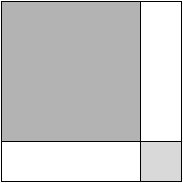
\includegraphics[scale=0.4]{FiguresMaths/proofa2plusb2}
\caption{A geometric proof of the identity $(n+1)^2 = n^2 + 2n + 1$.}
       \label{fig:proofa2plusb2}
\end{center}
\end{figure}
The figure tells its tale by exhibiting four rectangles that make up an $(n+1) \times (n+1)$ square; the area of this square is, of course, $(n+1)^2$.  This large square is made up of four rectangles.
\begin{itemize}
\item
Reading across the top of the figure, we encounter a darkly shaded $n \times n$ square (area $= n^2$) and an unshaded $n \times 1$ rectangle (area $= n$).
\medskip\item
Reading across the bottom of the figure, we encounter an unshaded $1 \times n$ rectangle (area $= n$) and a lightly shaded $1 \times 1$ square (area = $1$).
\end{itemize}
The overall message is that $(n+1)^2$ (the area of the large, composite, square)

\begin{tabular}{ll}
is the sum of & \\
  & \ $n^2$ \ (the area of the darkly shaded square) \\
plus & \\
  & $2n$ \ \ (the combined areas of the unshaded rectangles) \\
plus & \\
  & \ \ $1$ \ (the area of the lightly shaded square)
\end{tabular}

\medskip

\noindent
The preceding geometric validation does not ``look like'' the proofs whose highly structured forms we struggled with in high school.  But: (1) Our geometrical proof is as valid as any algebraic one; (2) It can be a lot more fun to come up with; (3) It may trigger reasoning that might lead to new discoveries.

\bigskip

\index{Al-Khw$\bar{\mbox{a}}$rizm$\bar{\mbox{i}}$!Muhammad ibn M$\bar{\mbox{u}}$s$\bar{\mbox{a}}$ al-Khw$\bar{\mbox{a}}$rizm$\bar{\mbox{i}}$}

\noindent {\it (ii) Solving a quadratic equation}.
We now develop a more complex example of pictorial reasoning.  The spirit of the following proof was provided by the 12th-century mathematician Al Khw$\bar{\mbox{a}}$rizm$\bar{\mbox{i}}$, whose seminal work \cite{Al-Khwarizmi} was indispensable in transmitting mathematical and computational ideas into Europe.  The following proof builds on his work on the second-degree equation
\begin{equation}
\label{eq:al-Khwarizimi}
x^2 + 10 x \ = \ 39
\end{equation}
The methodology that Al Khw$\bar{\mbox{a}}$rizm$\bar{\mbox{i}}$ employed for solving quadratic polynomial equations such as (\ref{eq:al-Khwarizimi}) builds solutions in terms of the areas of squares and rectangles and employs both algebraic and geometric representations of the lefthand sides of the target equations.  For equation (\ref{eq:al-Khwarizimi}) specifically, Al Khw$\bar{\mbox{a}}$rizm$\bar{\mbox{i}}$ found the perspicuous geometric representation of the lefthand side depicted in Fig.~\ref{fig:EqElKwarismi1}.
\begin{figure}[ht]
\begin{center}
       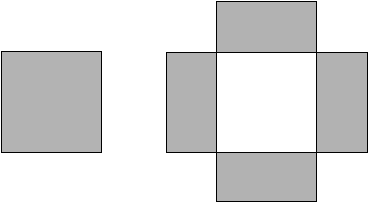
\includegraphics[scale=0.4]{FiguresArithmetic/EquationElKwarismi1}
\caption{The lefthand side of Eq.~(\ref{eq:al-Khwarizimi}) depicted geometrically via the shaded perfect square $x^2$ and (i.e., added to) four identical shaded rectangles of area $\frac{5}{2} x$ each.}
       \label{fig:EqElKwarismi1}
\end{center}
\end{figure}
In the figure, the shaded perfect square on the left and the unshaded perfect square on the right both have side $x$, hence, area $x^2$.  Of the four shaded rectangles around the unshaded perfect square, two have dimensions $\frac{5}{2} \times x$, and two have dimensions $x \times \frac{5}{2}$.  The figure's representation of the lefthand side of equation (\ref{eq:al-Khwarizimi}) is matched by the following rewriting of the lefthand side of (\ref{eq:al-Khwarizimi}):
\[ x^2 + 10 x \ \ = \ \ x^2 + \left( 4 \times \frac{5}{2} \right) x \]

We finally turn to solving the equation.
\begin{enumerate}
\item
The area of the entire shaded surface in Fig.~\ref{fig:EqElKwarismi1} is given by the righthand side of equation (\ref{eq:al-Khwarizimi}), that is $39$.
\medskip\item
Hence, $39$ is also the area of the ``cross'' on the righthand side of Fig.~\ref{fig:EqElKwarismi1} which would be created by moving the shaded $x \times x$ square into the unshaded $x \times x$ square.
\medskip\item
Finally, $39$ is also the area of the unshaded ``cross'' in Fig.~\ref{fig:EqElKwarismi2}.
\begin{figure}[ht]
\begin{center}
       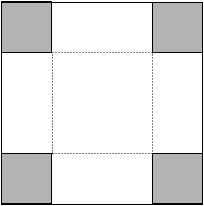
\includegraphics[scale=0.4]{FiguresArithmetic/EquationElKwarismi2}
\caption{The last step of the geometeric reasoning for solving the equation $x^2 + 10x = 39$.  The four shaded squares augment the area of the ``cross'' of Fig.~\ref{fig:EqElKwarismi1}, whose area equals $39$, to the the big square whose area equals $64$.}
       \label{fig:EqElKwarismi2}
\end{center}
\end{figure}
(The color scheme in this figure has been changed to highlight the new corner squares.)

\medskip\item
As in Fig.~\ref{fig:EqElKwarismi2}, let us append to the area-$39$ unshaded ``cross'' four small shaded squares whose addition augments the ``cross'' to the big, bi-color, square of
Fig.~\ref{fig:EqElKwarismi2}.

\medskip\item
We see from Fig.~\ref{fig:EqElKwarismi1} that each of the small shaded squares has dimensions $\frac{5}{2} \times \frac{5}{2}$, hence, area $25/4$.

This means that the area of the large square is
\[ 39 \ + \ \left( 4 \times \frac{5}{2} \right) \ = \ 39 + 25 \ = \ 64. \]
\end{enumerate}

\smallskip

We now have the information needed to compute a value of $x$ that satisfies equation (\ref{eq:al-Khwarizimi}).  Consider the large square of Fig.~\ref{fig:EqElKwarismi2}.

\begin{itemize}
\item
On the one hand, the side-length of this square is
\[ x \ + \ (2 \times 5/2) \ = \ x \ + \ 5 \]

\medskip\item
On the other hand, the side-length is
\[ x \ = \ 8 \]
\end{itemize}
Since all sides of the square are identical, we infer that
\[ x \ = \ 8-5 \ = \ 3 \]

\noindent
Indeed, we can---but do not need to!---verify this value algebraically.

\medskip

\noindent
{\em An important caveat}: The pictorial/geometric method which we have just employed is not ``complete''---it yields only the {\em positive} solution for $x$.  As we discuss at length in Sections~\ref{sec:fund-thm-algebra} and~\ref{sec:poly-by-radical}---see, in particular, Theorem~\ref{thm:fund-thm-algebra}---there exists another solution for $x$, because its defining polynomial is {\em quadratic} (i.e., of degree $2$).  In the light of the defining equation's intended goal---namely, to determine the area of a plot of land---the single (positive) solution for $x$ that Al Khw$\bar{\mbox{a}}$rizm$\bar{\mbox{i}}$'s tools yields was sufficient.  That said, there are situations wherein one has need of both roots of a quadratic polynomial equation, and the algebraic solution methods will produce both solutions---although not always in an intuitive way.

\medskip

Returning to equation (\ref{eq:al-Khwarizimi}):  the second, negative, solution for $x$  is $x' = -13$, as is witnessed by the following polynomial factorization:
\[ x^2 + 10x - 39 \ = \ (x-3)(x+13) \]
The serendipitous fact in this example is that, because $64$ is the square of $-8$, as well as of $+8$, {\em for this example}, the negative solution-value for $x$ can also be obtained via our geometric argument:
\[ x - 5 \ = \ -8 -5 \ = \ -13 \]
This aside, pictorial/geometric arguments can be fun to develop and can trigger unexpected discoveries!


\subsubsection{Handle pictorial arguments with care}

We have just mentioned one limitation of pictorial arguments, namely their limitation to certain types of problem solutions.  We now discuss an even more important reason to be careful when employing such arguments; the reason emerges from a paradox which is associated with the 19th-century British mathematician and fiction writer Lewis Carroll.
\index{(Lewis) Carroll's paradox} 
\index{Carroll, Lewis (pen name of Charles Lutwidge Dodgson)}

\medskip

Focus on a standard $8 \times 8$ chessboard.  Let us ``mutilate" the chessboard in the following way.
\begin{enumerate}
\item
Cut the board into four pieces in the manner specified schematically in Fig.~\ref{fig:LewisCarollParadox1}.
\begin{figure}[ht]
\begin{center}
       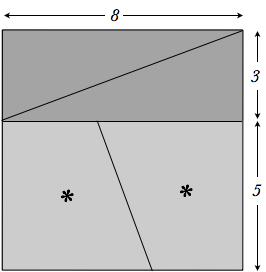
\includegraphics[scale=0.475]{FiguresMaths/LewisCarollParadox1}
\caption{A standard chessboard cut into four pieces.}
       \label{fig:LewisCarollParadox1}
\end{center}
\end{figure}
\medskip\item
Reassemble the four pieces into a rectangle in the manner depicted in Fig.~\ref{fig:LewisCarollParadox2}. 
\begin{figure}[ht]
\begin{center}
       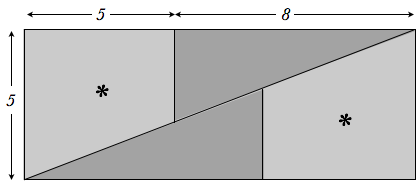
\includegraphics[scale=0.475]{FiguresMaths/LewisCarollParadox2}
\caption{The four pieces of the chessboard reassembled into a $5 \times13$ rectangle.}
       \label{fig:LewisCarollParadox2}
\end{center}
\end{figure}
\end{enumerate}

On the one hand, Fig.~\ref{fig:LewisCarollParadox1} supports assessing the {\em area} of the chessboard based on its conventional form, as an $8 \times 8$ array of unit-side squares.  Within this worldview, the board has {\em area} $8 \cdot 8 = 64$.

\smallskip

On the other hand, Fig.~\ref{fig:LewisCarollParadox2} supports viewing the chessboard in its cut-up-and-reassembled form.  In this worldview, the board has the area of a rectangular $5 \times 13$ array of unit-side squares is equal to $5 \times 13 = 65$.  Hence, within this worldview, the board has {\em area} $5 \cdot 13 = 65$.

\medskip

Obviously, something is wrong with our pictorial reasoning---but what?

\medskip

We can expose the problem by examining the southwest-northeast diagonal of the rectangle in Fig.~\ref{fig:LewisCarollParadox2} very carefully.  In the standard discussion of this ``paradox", the diagonal is drawn in a way that suggests that it is a line that {\em bisects} the $5 \times 13$ rectangle into two congruent (hence, equal-area) right triangles, and that this line is the shared hypotenuse of these triangles.  However, if one draws the figure in great detail, one finds that the diagonal does not quite bisect the rearranged unit-side squares of the $8 \times 8$ square!  In fact---see Fig.~\ref{fig:LewisCarollParadoxSol}---the pair of curves that actually bisect the rearranged $8 \times 8$ square {\em do not form a single line!}
\begin{figure}[ht]
\begin{center}
       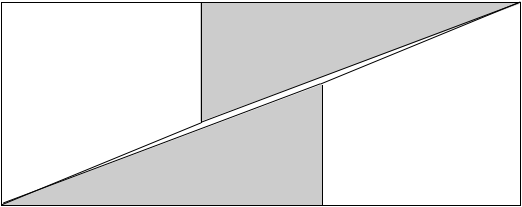
\includegraphics[scale=0.5]{FiguresMaths/LewisCarollParadoxSolution}
\caption{Looking carefully at the border between the northwestern and southeastern halves of the $5 \times 13$ rectangle.}
       \label{fig:LewisCarollParadoxSol}
\end{center}
\end{figure}
These two curves are really close to the diagonal, but they are separated by a {\em very small space}---indeed a space whose aggregate area equals the area of a unit-size square of the original $8 \times 8$ chessboard.

\bigskip

\noindent
{\bf The moral of this tale.}  Pictures can deceive as well as illuminate!  {\em Use pictures for inspiration---but always to verify that you are really seeing what you think you are!}


%{\Denis The complete explanation comes from the Cassini's identity, do you think we should refer to it here?}

%%%%%%%%%%%%%%%%%%%%%%%%%%%%%%%%%%%%%%%%%%%%%%

\subsection{Combinatorial Intuition and Argumentation}
\label{sec:comb-proofs}

Combinatorics is a branch of discrete mathematics that specializes in the following operations (among others): selecting objects from a given set; arranging and rearranging the objects; counting the number of ways that one can arrive at specified target configurations.
Chapter~\ref{ch:combinatorics} introduces the foundations of this subfield, following with its applications to the kindred fields of probability and statistics.

\subsubsection{Summation as a selection problem}
\label{sec:comb-sum-of-first-n}

Sometimes combinatorial argumentation can be used in unexpected ways.  We illustrate that fact here by   combinatorially deriving an explicit expression for the summation
$S_n \ \ = \ \ 1 \ + \ 2 \ + \cdots + \ n$.

Our summation begins, unexpectedly, by counting the number of ways---call it $C(n,2)$---of selecting two items from a set of $n$ items.  We describe this selection in a somewhat unconventional way.
\begin{itemize}
\item
The bigger integer of the two we are selecting can be chosen in $n$ ways, corresponding to the $n$ elements of the set
\[ \{ 1, \ 2, \ldots, \ n-1, \ n \} \]
\medskip\item
If the bigger item was integer $k$, then we can select the second, smaller, one in $k-1$ ways, from the integers smaller than $k$.
\end{itemize}
We thereby observe the following summation, which yields the desired value of $S_n$.
\begin{eqnarray*}
C(n,2) & = & n \ + \ \sum_{k=2}^n \ C(k-1,1) \\
       & = & n \ + \ \sum_{k=2}^n \ (k-1) \\
       & = & n \ + \ \sum_{k=1}^{n-1} \ k \\
       & = & S_n
\end{eqnarray*}

\subsubsection{Summation as a rearrangement problem}
\label{sec:summation-via-Fubini}

Our next proof technique is a combination of geometry and combinatorial rearrangement of a configuration of objects.  The second component of this pair incurs an intellectual debt to Guido Fubini, whose eponymous {\em Principle} mandates {\em looking at configurations from multiple points of view and garnering new intuitions from each}.
\index{Fubini, Guido} \index{Fubini's Principle}

\smallskip

We apply this two-stage reasoning paradigm to the problem of evaluating the summation $S_n \ = \ 1 + 2 + \cdots + n$.

\index{Gauss, Karl Friedrich}
\index{Gauss, Karl Friedrich!summation ``trick''}
The first idea in our reasoning is to represent each integer $k$ as a horizontal sequence of $k$ tokens, depicted as darkened circles in Fig.~\ref{fig:sumIntegers1}.
\begin{figure}[ht]
\begin{center}
       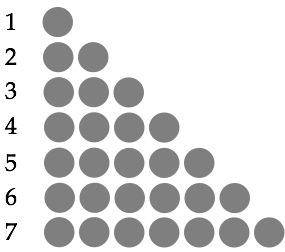
\includegraphics[scale=0.35]{FiguresMaths/SumIntegersBasis}
\caption{Representing the first $n$ integers using tokens.  In
  this illustration, $n=7$.}
       \label{fig:sumIntegers1}
\end{center}
\end{figure}
Using such a representation, we naturally view the summation $S_n$ as a \textit{triangular pattern} of tokens.  How can we use this representation to evaluate $S_n$ without just counting and summing?  We call upon an intuition attributed to the great 19th-century mathematician Karl Friedrich Gauss---who famously had this intuition as a pre-teenager.  We remark that if we {\em replicate} the triangular pattern in the figure and {\em flip} it, then we can configure the resulting triangles---see Fig.~\ref{fig:sumIntegers2}---to form the rectangular pattern depicted in Fig~\ref{fig:sumIntegers3}.
\begin{figure}[ht]
\begin{center}
       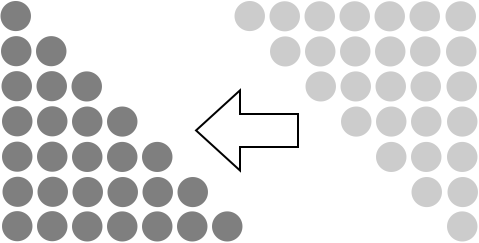
\includegraphics[scale=0.35]{FiguresMaths/SumIntegersIntermediate}
   \caption{Putting two copies of a triangle together to form a rectangle.}
       \label{fig:sumIntegers2}
\end{center}
\end{figure}
\begin{figure}[ht]
\begin{center}
       
\includegraphics[scale=0.35]{FiguresMaths/SumIntegersFinal}
\caption{The two copies of a triangle have become an $n \times (n+1)$
  rectangular array of tokens.}
       \label{fig:sumIntegers3}
\end{center}
\end{figure}
Next, we observe two important properties of the rectangular pattern that we have achieved in Fig~\ref{fig:sumIntegers3}.
\begin{itemize}
\item
The number of tokens in the rectangular pattern is precisely $2 S_n$.

\smallskip

This is a pictorial version of the seminal intuition that underlies Gauss's (text-based) summation of the series $S_n$; see Proposition~\ref{thm:sum-first-integers-Gauss}.

\medskip\item
The rectangular pattern has $n+1$ columns, each having $n$ tokens.

\smallskip

This means that the rectangular pattern contains $n \cdot (n+1)$ tokens.
\end{itemize}
Combining these observations, we conclude that
\[ 2 S_n \ = \ n \cdot (n+1) \ \ \ \ \mbox{ so that } \ \ \ \
S_n \ = \ {1 \over 2} n \cdot (n+1)
\]


\subsection{The Computer as a Mathematician's Assistant}

Computers have played an essential role in the process of ``doing'' mathematics from the earliest times when computers had enough power to explore the mathematical terrain, searching and verifying.
\begin{itemize}
\item
Some of the calculations performed by these ``silicon assistants'' have a game-like quality to them:
  \begin{itemize}
  \item
Calculate more digits of $\pi$ than anyone else has done
  \medskip\item
Calculate a bigger Mersenne prime than anyone else has
  \end{itemize}

\medskip\item
Yet other calculations represent attempts to hone intuition for what will someday morph into serious attempts at proofs:
  \begin{itemize}
  \item
Search for an odd perfect number
  \medskip\item
Determine the relative frequencies of the decimal digits in the infinite decimal expansion of $\pi$
  \end{itemize}

\medskip\item
Finally, some of these calculations represent attempts to contribute essential details to already-serious attempts at proofs: These are our interest here.
\end{itemize}

Many significant theorems languished as conjectures for decades, some even for centuries, awaiting elevation to theoremhood.  While many of these eventual theorems languished in mathematical limbo as they awaited the development of new mathematics---Fermat's Last Theorem (Theorem~\ref{thm:Fermat-last}) is a prime example---yet others have suffered their fates because of a plethora of cases that needed (often-minor) calculational verification.

The latter category of conjecture can increasingly be tackled with the aid of the ever-more powerful computers that are being developed with ever-increasing frequency.  When used in this way, computers are clearly ``junior'' partners to their mathematican-users.  When the domain of discourse within a conjecture is discrete---i.e., does {\em not} involve real numbers ``to infinite precision'' nor any continuity-related notions---then it is always possible---at least in principle---to eliminate the computer from the ``team'' by transforming such a verification into a classical formal proof.  The role of the computer in the ``team'' is solely to assist the mathematicians---by
performing calculations that are too long and/or too numerous and/or too complicated for humans to perform reliably and efficiently.

 \index{Appel, Kenneth} \index{Haken, Wolfgang}
The renowned Four-Color Theorem (Theorem~\ref{thm:Four-ColorTheorem}) was a landmark in the use of computers as partners to humans in proving theorems.  The Theorem asserts---ignoring a few technical details---that any map on Earth (or on a topologically similar planet) can be colored using four colors in such a way that distinct countries that share a border receive distinct colors.  As we discuss in some detail in Section~\ref{sec:planar+outerplanar-color}, this result languished in mathematical limbo for many decades before a pair of American mathematicians, Kenneth Appel and Wolfgang Haken, used a computer to help resolve the thousands of cases that had to be verified-via-calculation in the proof.

The mathematical world erupted in controversy over this first-ever use of a computer in an essential way to construct a mathematical proof.  It took years---plus the result-replicating program of a team of Japanese mathematicians---before the global mathematical community accepted the claim by Appel and Haken that Theorem~\ref{thm:Four-ColorTheorem} had, indeed, been proved!

\medskip

There may be many conjectures currently in mathematical limbo that could be elevated to the status of theorem if some team of mathematicians would feel free to employ computers to offload needed but onerous computational drudgery.


%%%%%%%%%%%%%%%%%%%%%%%%%%%%%%%%%%%%%%%

\section{Exercises: Chapter 2}

Throughout the text, we mark each exercise with 0 or 1 or 2 occurrences of the symbol $\oplus$, as a rough gauge of its level of challenge.  The 0-$\oplus$ exercises should be accessible by just reviewing the text.  We provide {\em hints} for the 1-$\oplus$ exercises; Chapter~\ref{ch:Exercises} provides {\em solutions} for the 2-$\oplus$ exercises.  Additionally, we begin each exercise with a brief explanation of its anticipated value to the reader.

\begin{enumerate}
\item
{\bf Verifying some summations via Finite Induction}

{\sc Lesson:} Practice using Induction plus some algebraic calculation

\smallskip

{\em Use Finite Induction to verify that the following summation formulas hold for all positive integers $n$.}
  \begin{enumerate}
  \item
Summing the first $n$ fixed powers of integers.
       \begin{enumerate}
       \item
$S_2(n) \ \ \eqdef \ \ 1 + 2^2 + \cdots  + n^2 \ \ = \ \ {1 \over 6} n (n+1)(2n+1)$

     \medskip\item
$S_3(n) \ \ \eqdef \ \
1 + 2^3 + \cdots  + n^3 \ \ = \ \
\frac{1}{4} n^2 (n+1)^2$
    \end{enumerate}
Note that the sum of the first $n$ integers is quadratic (degree $2$) in $n$ (Proposition~\ref{thm:sum-1-to-n-induction1}); the sum of the first $n$ squares of integers is cubic (degree $3$) in $n$; the sum of the first $n$ cubes of integers is quartic (degree $4$) in $n$.  Do you detect the pattern?  {\em New mathematics is born from such detected patterns!}  We shall verify this pattern in Chapter~\ref{ch:Summation}.

  \medskip\item
Summing the first $n$ powers of a fixed base number (we use base $2$).
       \begin{enumerate}
       \item
$\sum_{i=0}^n \ 2^i \ \ = \ \ 1 \ + \ 2 \ + \ 4 \ +  \cdots + \ 2^n \ \ = \ \ 2^{n+1} -1$
       \medskip\item
$\sum_{i=0}^n \ i 2^i \ \ = \ \ 2 \ + \ 8 \ + \ 24 \ +  \cdots + \ n 2^n \ \ = \ \
n 2^{n+1} \ + \ 2$
    \end{enumerate}
Note that exponential grow so fast (as functions of $n$) that the sum of terms is just a bit larger than the largest term!  We shall learn, in detail, how to discover this fact in Chapter~\ref{ch:Summation}.

\ignore{*********
\medskip\item

Prove $F_{k-1}.L_n = F_{n+k} - (-1)^k F_{n-k}$, $\forall 1 \leq k \leq n$

where $F$ and $L$ and respectively Fibonacci and Lucas numbers.

The basis case of the induction is for $k=1$
*********}
  \end{enumerate}


\medskip\item
$\oplus$
{\bf Meeting people at a party}

{\sc Lesson:} Experience using the Pigeonhole Principle

\smallskip

You are attending a cocktail party that is populated by $n$ couples.  Attempting to create a warm atmosphere, the host requests that each attendee shake the hand of every attendee that he or she does not know.

\smallskip

{\em Prove that some two attendees shake the same number of hands.}
\medskip

\medskip\item
{\bf An elementary result about encoding}

{\sc Lesson:} Practice using Proof by Contradiction

\smallskip

Here is a simple way to encode an ordered pair of positive integers as a single positive integer.

\smallskip

{\em Prove the following assertion using a proof by contradiction.}

\begin{prop}
Let $a, b, c, d$ be (not necessarily distinct) positive integers.

If $2^a 3^b \ = \ 2^c 3^d$, then $a=c$ and $b=d$.
\end{prop}

\medskip\item
$\oplus$
{\bf Bi-colored necklaces in tubes}

\index{Rolle's Theorem} \index{Rolle, Michel}

{\sc Lesson:} The nature of gradual transitions---a discrete analogue of {\em Rolle's Theorem} {\small (Michel Rolle, 1691)}

\smallskip

{\small\sf Purely mathematical, continuous, version}:
You start at point $A$, carrying $w_1$ units of load. You move toward point $B$, shedding load at a steady pace.  {\em If you reach point $B$ with $w_2$ units of load, then at some point in your journey, you had ${1 \over 2} (w_1 + w_2)$ units of load.}

\smallskip

{\small\sf Discrete version in a ``real" setting}.
You have a {\it necklace} composed of $2n$ jewels: $2a$ black jewels and $2b$ white jewels.  For illustration, the necklace in Fig.~\ref{fig:sample-necklace} has $n = 6$, $a = 5$, and $b =1$.
\begin{figure}[ht]
\begin{center}
       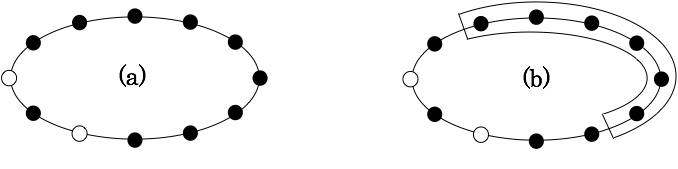
\includegraphics[scale=0.35]{FiguresMaths/SampleNecklace}
\caption{(a) A necklace having $12$ jewels: $10$ black and $2$ white.  (b) The necklace in a tube.}
\label{fig:sample-necklace}
\end{center}
\end{figure}
In part (a) of the figure, the necklace is unadorned; in part (b), the necklace appears within a length-$n$ {\it tube} which isolates one string---i.e., half-necklace---of $n$ jewels from the complementary string.

\smallskip

{\em Prove the following.}

\begin{prop}
For any bi-colored necklace of the form described---i.e., with even numbers of jewels, black jewels, and white jewels---there is a way to position the tube so that inside the tube and outside the tube, there are equally many jewels, equally many black jewels, and equally many white jewels.
\end{prop} 

\smallskip

{\em Hint}: Slide the tube around the necklace, and count both black and white jewels at each step.  How can these numbers change in a single step?
\medskip

\medskip\item
{\bf There is only one $1$ (as a multiplicative identity)}

{\sc Lesson:} There is precisely one multiplicative identity for the integers.

\smallskip

{\em Prove the following assertion by contradiction.}

\begin{prop}
The integer $1$ is the unique multiplicative identity for the integers.  In other words, if the positive integer $a$ satisfies {\em either} the equation
\[ a \times x \ = \ x \]
{\em or} the equation
\[ x \times a \ = \ x \]
for all positive integers $x$, then $a = 1$.
\end{prop}

\medskip\item
{\bf $\oplus$ Using {\em geometric} intuition to sum inverse powers of $4$}

{\sc Lesson:} Exploiting geometric intuition toward a sophisticated end.

\smallskip

We turn to a variant of Proposition~\ref{thm:sumof-1/4-induction}.  This time, we focus on the entire infinite summation
\[ S \ \ = \ \  {1 \over 4} \ + \  {1 \over 4^2} \ + \cdots + \ {1 \over 4^k} \ + \cdots  \]
and we do so from a geometric point of view.

\smallskip

We prove in Proposition~\ref{thm:sum-finite-geometric-series}(b) that this infinite summation converges to the value ${1 \over 3}$.  A simple way to see this is to multiply the summation $S$ term by term by the fraction $1/4$.  We observe---just by inspection---that the resulting product, which clearly has the value $S/4$, equals $S - 1/4$, so that $S = 1/3$.

\smallskip

There is a charming geometric argument which mimics the preceding conversion of the original summation into a quarter-valued version of itself, followed by a summarizing calculation.  This argument exposes in a compelling way the {\em self-similarity} which underlies the argument.  We get you started on this argument in Fig.~\ref{fig:Sum1over4}.
 \begin{figure}[ht]
\begin{center}
       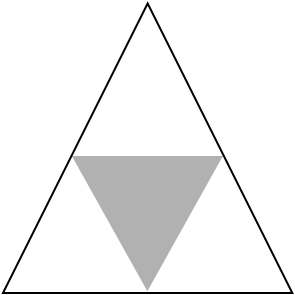
\includegraphics[scale=0.35]{FiguresMaths/Sum1over4}
\caption{Partitioning a unit-area isosceles triangle into $4$ sub-triangles, each of area $1/4$.}
       \label{fig:Sum1over4}
\end{center}
\end{figure}
Observe that we can iterate the partitioning process in the figure on any one of the four sub-triangles of the original triangle---because all four sub-triangles are identical to each other (except for placement and orientation) and are similar to the original triangle.

\smallskip

We have now described the process at a very high level.  Your assignment is to flesh out the details.  {\em Prove that the four sub-triangles
\begin{itemize}
\item
are similar to one another
\medskip\item
are similar to the original triangle
\medskip\item
have area which is $1/4$ that of the original triangle
\end{itemize}
Assemble these facts into an evaluation of the sum $S$.}
\end{enumerate}


\ignore{******************
%%%%%%%%%%%%%%%%%%%%%%%%%%%
%%%%%%%%%%%%%%%%%%%%%%%%%%%
%%%%%%%%%%%%%%%%%%%%%%%%%%%

\subsection{A graphical proof}

\noindent \textit{The aim.}
Use a pictural argument to prove a nonobvious identity of arithmetic sums
that one would be unlikely to come upon by purely textual thinking.
\medskip

\noindent \textit{The problem.}
%\label{thm:an-arithmetic-identity}
Prove the following property:

for any positive integer $n$,
\[ \Delta_{2n-1} \ = \ n + 4 \Delta_{n-1}. \]
\medskip

\noindent \textit{Hint.}
Consider the arithmetic series for the case
$a=1$ and $b=4$ (see~\ref{eq:arith-seq} for more details) whose result is:
\begin{equation}
\label{eq:triangles}
S^{(1,4)}(n) \ = \ n + 4 \Delta_{n-1}.
\end{equation}
Represent the sum $\Delta_{n-1}$ as a triangle of tokens and put those four as a larger triangle.
\medskip

\noindent \textit{Lesson learned.}
Mastering graphical proofs.


\subsection{A variant for computing the sum of the first integers $\Delta_n$}

\noindent \textit{The aim.}
Application of geometric sum.
\medskip

\noindent \textit{The problem.}
%Compute the sum of the first integers $\Delta_n$. 
Show graphically that $\Delta_n$ (sum of the first $n$ integers) is congruent to $1$ modulo $8$.
\medskip

\noindent \textit{Hint.}
Write the previous relation as $8 \Delta_n = K^2 -1$
for an integer $K$ (to be determined) and represent the square $K$ by $K$. 
\medskip

\noindent \textit{Lesson learned.}
Mastering geometrical proofs.




%%%%%%%%%%%%%%%%%%%%%%%%%%%%%%%%%%%%%%%

\subsection{A graphical proof for a specific geometric series}

\noindent \textit{The aim.}
To develop more intuition in solving using geometrical arguments.
\medskip

\noindent \textit{The problem.}
Compute the sum of $(\frac{1}{4})^k$ using a graphical argument ($k \geq 0$).
\medskip

\noindent \textit{Hint.}
A rapid analysis of the small values of $k$ leads to the guess $(\frac{1}{4})^k = \frac{1}{3}$.
The solution is to generalize Fig.~\ref{fig:Sum1over4}.
 \begin{figure}[ht]
\begin{center}
       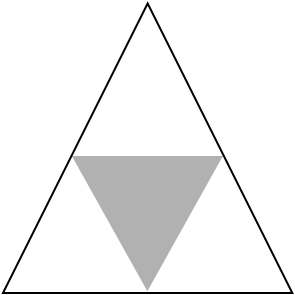
\includegraphics[scale=0.4]{FiguresMaths/Sum1over4}
\caption{Division of a isosceles triangle of surface $1$ into $4$ equal pieces.}
       \label{fig:Sum1over4}
\end{center}
\end{figure}
\medskip

\noindent \textit{Lesson learned.}
Training and gain intuition for mastering geometrical proofs. 
***************}
